\subsection*{Divide and Conquer}
The problem is \textbf{divided} into smaller subproblems. If the subproblems are
large enough to be solved recursively, we call that the \textit{recursive case}.
Once the problem is too small, the recursion \textit{bottoms out} and we are at
the \textit{base case}. We can no longer recurse, and we solve the problem.
Sometimes the subproblems looks different than the original problem on top of
having to solve smaller instances of the same problem. This is the \textbf{conquer}
step. Lastly we \textbf{combine} the subsolutions and the original prolem is
solved.

\subsection*{Mergesort}
\textbf{Divide:} divides the sequence of size $n$ into two subsequence of size
$n/2$.\newline
\textbf{Conquer:} Sort the subsequences recursively until the sequences have
size $1$, in which case the subsequence is sorted.\newline
\textbf{Combine:} We merge the two sorted subsequences, making sure that they
appear in the correct order.
\newline\newline
The key operation in \texttt{Mergesort} is the combine step, where \texttt{Merge}
is called, since \texttt{Merge} merges two already sorted subsequences, and
ensures that the resulting merged sequence is sorted as well.

\subsubsection*{Example}
\begin{forest}
  for tree={
    draw,
    align=center
  }
  [$1$ $10$ $5$ $8$ $3$ $10$
    [$1$ $10$ $5$
      [$1$ $10$
        [$1$]
        [$10$]
      ]
      [$5$
        [$5$]
        [$\infty$]
      ]
    ]
    [$8$ $3$ $10$
      [$8$ $3$
        [$8$]
        [$3$]
      ]
      [$10$
        [$10$]
        [$\infty$]
      ]
    ]
  ]
\end{forest}
\newline\newline
\begin{forest}
  for tree={
    draw,
    align=center
  }
  [$1$ $3$ $5$ $8$ $10$ $10$
    [$1$ $5$ $10$ $\infty$
      [$1$ $10$ $\infty$
        [$1$ $\infty$]
        [$10$ $\infty$]
      ]
      [$5$ $\infty$
        [$5$ $\infty$]
        [$\infty$]
      ]
    ]
    [$3$ $8$ $10$ $\infty$
      [$3$ $8$ $\infty$
        [$8$ $\infty$]
        [$3$ $\infty$]
      ]
      [$10$ $\infty$
        [$10$ $\infty$]
        [$\infty$]
      ]
    ]
  ]
\end{forest}

$\infty$ is not in the final sequence since the last \texttt{for}-loop in
\texttt{Merge} only iterates for every element in the final sequence. That is
also why there is only one $\infty$ symbol for each subsequence.

\subsubsection*{Runtime $\Theta(n\log n)$}
The runtime of a \textbf{Divide-and-Conquer} algorithm is calculated as such:
\begin{align*}
  T(n)=
  \begin{cases}
    \Theta(n)&\textrm{ if }n\leq c\\
    aT(n/b)+D(n)+C(n)&\textrm{ otherwise.}
  \end{cases}
\end{align*}
\texttt{Merge} runs in $\Theta(n)$ time since at most $n$ basic steps are
performed. \texttt{Mergesort} find \textbf{divides} the problem by finding the
middle of the array. This happens in constant time. $D(n)=\Theta(1)$.
\newline\newline
Since the algorithm is \textbf{conquered} there are two recursive calls, each of
which represent half of the original problem, we have $2T(n/2)$.
\newline\newline
\texttt{Merge} \textbf{combines} the subsolutions. If \texttt{Merge} is called
with a sequence of size $n$, then $C(n)=\Theta(n)$.
\newline\newline
See recursion tree on the next page.
\begin{align*}
  T(n)=
  \begin{cases}
    \Theta(1)&\textrm{ if }n=1\\
    2T(n/2)+\Theta(n)&\textrm{ if }n>1.
  \end{cases}
\end{align*}
\begin{figure}[H]
  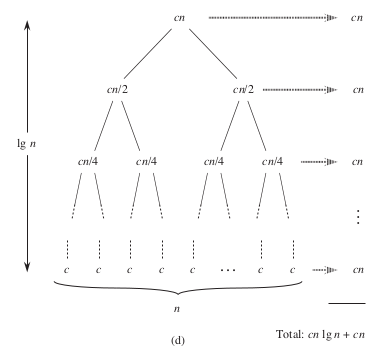
\includegraphics[scale=0.75]{pictures/recursiontree.png}
  \caption{Recursion tree of \texttt{Mergesort}}
\end{figure}
\iffalse
\makecomment{If there is time - show by substitution}\newline\newline
\textit{Guess:} $T(n)=O(n\lg n)$
\newline\newline
The want to find an upper bound on the recurrence
\begin{align*}
  T(n)=2T(\lfloor n/2\rfloor)+n
\end{align*}
We assume that this bound holds for all $m<n$ where $m=\lfloor n/2\rfloor$. We
write:
\begin{align*}
  T(n)&\leq\textrm{ }2(c\lfloor n/2\rfloor\lg(\lfloor n/2\rfloor))+n\\
  &\leq\textrm{ }cn\lg(n/2)+n\\
  &=\textrm{ }cn\lg n-cn\lg2+n\\
  &=\textrm{ }cn\lg-cn+n\\
  &\leq\textrm{ }cn\lg n\\
  \floor{n}
\end{align*}
\fi

\subsubsection*{Correctness: Proof by loop invariant}
In Mergesort the \textbf{combine} step solves the problem, and thus the
correctness of \texttt{Merge} will be proved.\newline\newline
We wish to maintain the following loop invariant. 
